\documentclass[12pt]{article}\usepackage[]{graphicx}\usepackage[]{color}
%% maxwidth is the original width if it is less than linewidth
%% otherwise use linewidth (to make sure the graphics do not exceed the margin)
\makeatletter
\def\maxwidth{ %
  \ifdim\Gin@nat@width>\linewidth
    \linewidth
  \else
    \Gin@nat@width
  \fi
}
\makeatother

\definecolor{fgcolor}{rgb}{0.345, 0.345, 0.345}
\newcommand{\hlnum}[1]{\textcolor[rgb]{0.686,0.059,0.569}{#1}}%
\newcommand{\hlstr}[1]{\textcolor[rgb]{0.192,0.494,0.8}{#1}}%
\newcommand{\hlcom}[1]{\textcolor[rgb]{0.678,0.584,0.686}{\textit{#1}}}%
\newcommand{\hlopt}[1]{\textcolor[rgb]{0,0,0}{#1}}%
\newcommand{\hlstd}[1]{\textcolor[rgb]{0.345,0.345,0.345}{#1}}%
\newcommand{\hlkwa}[1]{\textcolor[rgb]{0.161,0.373,0.58}{\textbf{#1}}}%
\newcommand{\hlkwb}[1]{\textcolor[rgb]{0.69,0.353,0.396}{#1}}%
\newcommand{\hlkwc}[1]{\textcolor[rgb]{0.333,0.667,0.333}{#1}}%
\newcommand{\hlkwd}[1]{\textcolor[rgb]{0.737,0.353,0.396}{\textbf{#1}}}%
\let\hlipl\hlkwb

\usepackage{framed}
\makeatletter
\newenvironment{kframe}{%
 \def\at@end@of@kframe{}%
 \ifinner\ifhmode%
  \def\at@end@of@kframe{\end{minipage}}%
  \begin{minipage}{\columnwidth}%
 \fi\fi%
 \def\FrameCommand##1{\hskip\@totalleftmargin \hskip-\fboxsep
 \colorbox{shadecolor}{##1}\hskip-\fboxsep
     % There is no \\@totalrightmargin, so:
     \hskip-\linewidth \hskip-\@totalleftmargin \hskip\columnwidth}%
 \MakeFramed {\advance\hsize-\width
   \@totalleftmargin\z@ \linewidth\hsize
   \@setminipage}}%
 {\par\unskip\endMakeFramed%
 \at@end@of@kframe}
\makeatother

\definecolor{shadecolor}{rgb}{.97, .97, .97}
\definecolor{messagecolor}{rgb}{0, 0, 0}
\definecolor{warningcolor}{rgb}{1, 0, 1}
\definecolor{errorcolor}{rgb}{1, 0, 0}
\newenvironment{knitrout}{}{} % an empty environment to be redefined in TeX

\usepackage{alltt}
\usepackage[utf8]{inputenc}
\usepackage{graphicx}
\usepackage{subfigure}
\usepackage{multicol}
\usepackage{lipsum}
\usepackage{mwe}
\usepackage{gensymb}
\usepackage{setspace}
\usepackage{natbib}

\usepackage[margin=1 in]{geometry}
\usepackage{cite}
\usepackage{natbib}
\bibliographystyle{..//refs/styles/besjournals.bst}

\title{Thermo- vs. Photo-periodicity}
\author{D Buonaiuto, M Donahue, EM Wolkovich}
\date{March 2019}
\IfFileExists{upquote.sty}{\usepackage{upquote}}{}
\begin{document}

\maketitle
\begin{enumerate}
    \item Introduction
    \begin{enumerate}
        \item Phenology is important
        \item Experiments show phenology cued by temperature and photoperiod.
        \item Interactions are important and need to be pursued.
         \item Testing interactions is complex; we will consider photoperiod and forcing
        \item Must be orthogonal
    \end{enumerate}
    \item Experimental Designs for interactions
    \begin{enumerate}
        \item Each cue has possible 2 axes, intensity and period.
        \begin{enumerate}
            \item Photoperiod: usually concerned with period only
            \item Forcing, both period and intensity (temperature)
        \end{enumerate}
        \item Three major experiment designs could be utilized.
        \begin{enumerate}
            \item Temp intensity and photo period
            \begin{enumerate}
                \item Pro: Simple, easy to make truly orthogonal
                \item Con: Some literature says this is bad for temperature. (find it). As such is rarely done.
            \end{enumerate}
            \item Covary thermo- and photo-period (most common).
            \begin{enumerate}
               \item Pro: more accurate representation of forcing. Simulates nature so good for comparison to field.
                \item Con: Non-orthogonal for GDH. Can determine between photo-period and thermo-period effects.
            \end{enumerate}
          
            \item Decouple thermo- and photo-period (never really done).
            \begin{enumerate}
                \item Pro: Orthogonal for GDH.
                \item Con: New Non-orthogonal issue. Dawn T. (Find citations)
            \end{enumerate}
        \end{enumerate}
        \item Design II will probably continue to be most popular. And we can and should use math to more accurately interpret our results.
    \end{enumerate}
    \item Mathematical Predictions
    \begin{enumerate}
        \item Explain Data
        \item Assumptions
        \begin{enumerate}
            \item Forcing is most important
            \item Others
        \end{enumerate}
        \item Show the math
        \item make predictions
    \end{enumerate}
    \item Experimental Validation
    \begin{enumerate}
        \item Explain experiment two.
        \item Present comparison results
    \end{enumerate}
\end{enumerate}


\section*{Introduction}

 \indent \indent Phenology, the timing of life cycle transitions in organisms, is important component of ecosystem structure and function \citep{Chuine2001, Piao2007,Cleland2007}. While phenology has been of interest to biologists for over a century, it has begun to receive increased attention in the recent decades as observed phenological shifts across a broad taxonomic spectrum have emerged as one of the most widely observed effects of anthropogenic climate change to date \citep{Parmesan2003,Root2003,Menzel2006,Wolkovich2014}. \\
\indent It has long been recognized that experimental manipulations in artificial environments are ideal for mechanistically characterizing phenological response to environmental fluctuations \citep{Ettinger_inprep,Primack2015}. This body of experimental work has demonstrated that temperature (winter chilling and spring forcing) and photoperiod are the primary cues of phenology for plants in the temperate/boreal zones \citep{Rathcke1985,Visser2010,Forrest2010}.\\
\indent Recent advances have demonstrated that plant phenological responses are nonlinear, due largely to interactions between cues\citep{Flynn2018,Laube2014}. This highlights the need for experiments to be designed to evaluate the strength of these interactions. To truly test interactions, treatments must be orthogonal: that is there must be more than one level of each treatment, and each level of each treatment must be crossed with every level of the other. This adds complexity to experimental setups, and experimental artifacts that interfere with interpretation of results are readily introduced \citep{Wolkovich2012}. In this paper, we discuss a particular challenge that arises when investigation interaction between forcing temperate and photoperiod.

    \section*{Considering light and temperature in phenology experiments}
 \indent \indent  For both light and temperature cues, there are two axes that can be manipulated in experiments. Then intensity of the cue (ie temperature of forcing or light intensity/wavelength) and the period (duration of temperature exposure or light periods). While light intensity has been to shown to affect many aspects of organism's biological activity including phenology \citep{Brelsford2018,Cober1996}, the period of light exposure is generally considered to be the dominate light cue, and phenological research interests tends to focus on photoperiod rather than intensity \citep{findcitations}. For temperature, though intensity is considered a major driver of phenology, the very common and successful model framework for quantifying temperature effects on phenology, the growing degree day or growing degree hour, integrates temperature with its period. Researchers must be thoughtful about how to incorporate these three main treatment axes(photo-period, theromo-period and thermo-intensity) in their experiments, and be wary of how these decisions will affect their experimental inference. There are three basic experimental designs (see figure \ref{fig:Figure 1} which are detailed in brief below:
\subsubsection*{Manipulation of Temperature intensity and photoperiod:}
\indent \indent The most simple design to test for a temperature x light interaction is to manipulate only one axis of each cue, for example, temperature intensity and light period. This would be implemented by applying high and low forcing treatments at constant temperatures, and crossing these with a long and short photo-period treatment at a constant light intensity (figure \ref{fig:Figure 1}a).\\
\indent The main advantage of this design is that is it simple to implement, maintains the orthogonality among the four treatment combinations (warm/short, warm/long, cool/short, cool/long) and allows for a very straight forward interpretation of the predictors. Additionally some studies have found that leaf expasion is faster at constant temperatures when compared to diurnally fluctation thermoperiods \citep{Erwin1995}. However,in nature, plants experience substantial diurnal temperature variation, and as such, growth chambers experiments without a diurnal thermoperiod would be a poor approximation of natural conditions. Other studies indicated that species may infact be responding to the differences between day and night temperatures \citep{Erwin1995},which raises futher questions about the utility experiments lacking thermoperiodicty for understanding the ecology and evolution of play in nature. On account of these shortcomings, it has become quite standard for researchers to include a diurnally varying thermo-period for forcing treatments. For example, rather than static high/low forcing treatments of 20\degree C and 16\degree C, researchers would use, a high forcing treatment of 24\degree/16\degree C and low 20\degree/12\degree C (day/night). \citep{Ettinger_inprep}.
\subsubsection*{Coupled photo- and thermo-periodicity:}
\indent\indent Incorporating diurnal thermo-periodicity into experimental design require that researcher decide how to vary this periodicity relative to the experiments photo-period cycle. The vast majority of published experiments employ a design in which photo-and thermo-periodicity are synchronized as in (figure \ref{fig:Figure 1}a) \citep{Ettinger_inprep}. This design is perhaps the most intuitive, one,  following the fact the photo- and thermo-period tend to co-vary in nature \citep{findcitations}. This approximation of natural conditions may make this design the most useful for extrapolating inferences between experimental and observational studies. However, while it appears, to maintain orthogonality between treatments when considering temperature intensity alone, but, in this case, the forcing response is a product of both the intensity of the temperature cue and the duration of its exposure (growing degree hours).  Thus, the coupling of photo- and thermo-period results in non-orthogonality between the four treatment combinations (see figure \ref{fig:Figure 2}a). In this scenario, the effect of photo-period cannot be neatly distinguished from the effects of increased thermo-period under the longer day treatments, making it impossible to accurately evaluate the relative importance of these cues, which is often a a major goal of growth chamber experiments. This results in spurious interpretation of experimental result.
\subsubsection*{Decoupled photo- and thermo-periodicity:}
 \indent \indent An alternative experimental design that incorporates thermo-periodicity into a temperature x photoperiod interaction experiment is decouples the experimental thermo- and photo- periods. The would be achevied by varying thermo-period on a constant schedule across all four treatment combinations (figure \ref{fig:Figure 1}c). Though this experiment set up has not be widely, if ever, employed in growth chamber experiments \citep{Ettinger_inprep}, this design restores full orthogonality to growing degree hour sums that make up the forcing treatment (figure \ref{fig:Figure 2}a).\\
\indent But this obvious advantage for reasonible statistical comparisons introduces a new biological artifact that may bias experimental results. Evidence from horticulture studies have demonstrated that cell growth is most sensitive to temperature fluctuation at the beginning of the photoperiod\citep{Erwin1998}. This suggests that dawn temperatures may be disproportionatly strong driver biological activity in plants. For example,it has been shown that that increasing temperatures in the first two hours of the photoperiod was almost as effective for stimulating shoot elongation as similar temperature increases for the whole photoperiod \citep{Erwin1998}. These results have been supported more generally by the observation that phenology is more response to daytime warming that night \citep{Rossi2017}. By de-coupling thermo-period from the photo-period manipulations, experimenters by neccesity introduce an assymetry between the photoperiod treatments \textit{relative} to the thermoperiod. In our example in \ref{fig:Figure 1}c), the long and short day photoperiod treatments have the same 12 thermoperiodicity cycle, but in the long day treatments, the plant does not experience "day time" temperatures until after they encounter "day light", while the plants in the short day treatment experience day time warming before light.\\
\indent Given the demonstrated importance of the interaction between temperature and photoperiod at dawn, it could be suggested that a design that the one depicted in figure \ref{fig:Figure 1}d in and improved version of a uncouple thermo and photo period design, because the temporal relationship between dawn light and temperature is standardized across all treatments, but this again produces an unreasilstic comparision with nature, and the "true" effects of warming may be obscured by that fact for the short day treatments, there is less overlap between day time temperature and light conditions.\\ %%% I am acutally slowly convincing myself that this design is superior and should be used
\indent As we have shown above, each design introduces its own biological or statistical artifacts that will bias he results of the experiments. We cannot conclusively solve the problems of true inference through modifying experimental designs, but rather, we must thoughtful incorporate the implications of these design choices into our statistical metrics and interpretation of results. While we cannot conclusively suggest a optimal experimental design, we expect that because of its history and relationship to field conditions, a coupled photo-and thermo- period design will remain the most popular choice for phenological experiments in artificial environments. In the following section, we will use a public dataset to demonstrate how mathematical principles can be applied to tease apart the artifact introduced by this inherently imperfect experimental design and make more meaningful inferences about the cue interactions. 


\section*{Math}   
\indent\indent  Our analysis is based on results from a large scale growth chamber experiment by \citet{Flynn2018}, in which in addition to chilling and provenance, fully factorial light and temperature manipulations were applied to twig cuttings from 28 woody species. The authors determined a mean budburst  sensitive to temperature of -9.5, and  a mean sensitivity to photo-period of -4.5 with a weak, negative interaction between the two cues. We set out to calculate how much of the reported photo-period response could in actuality be driven by the latent differences in thermo-period between the long and short photo-period treatments. 
    \begin{enumerate}
    \item  State some assumptions. IE forcing is dominant cue
        \item Do some math
        \item  Make a prediction.
    \end{enumerate}



\section*{Validation}
\indent\indent The prediction presented in the previous section could be re-phased as the expected difference in photoperiod sensitive between a coupled and decoupled photo- and thermo-period experiment with all other treatment levels held equal. While we are aware of no experiments that have explicitely set out to test such predictions, we now present a previously unpublished dataset from Buonaiuto and Wolkvich (20someday) that allows us to empirical test our predictions stated above. The Buonaiuto and Wolkovich study applied serveral treatments levels that overlap with those in the \citet{Flynn2018} study to twig cuttings from the same source population, but in this trial, photo- and thermo-period were decoupled. A comparative reanalyses of these revealed at a given equal forcing temperature, differences in the photo-period effect, attribuated to the alternative  periodicities designs, were on the same order as those predicted above for both bud burst and leaf out for the group of species common between the two experiments.


\begin{enumerate}
  \item How do we know if this is a good prediction? We are essentially predicting the expected difference between experimental design two and three.
\item We have 2 dataset. A subset of a \citet{Flynn2018} study were sampled  at Harvard Forest,  were forced at 18 day 12 night, with photoperiod treatments of 8 and 12 hours. 
\item Another experiment by Buonaiuto and Wolkovich (unpublished data) also included these treatment levels, But, decoupled thermo-and photo-periodicity. What a happy accident.
\item We reanalyzed these datasets to compare the effects of coupling vs. uncoupling, see \ref{fig:Figure 2}.

\end{enumerate}
 
 \section{Wrap up}
 \begin{enumerate}
\item We can't say which design is absolutely best.
\item We expect design 2 will remain popular. This is okay because we have shown the design flaws are easiest to overcome mathematically.  
\item We externally validated the math
\item Future studies should do this.
 \end{enumerate}

 \bibliography{..//refs/periodicity.bib} 

\begin{figure}[h!]
    \centering
 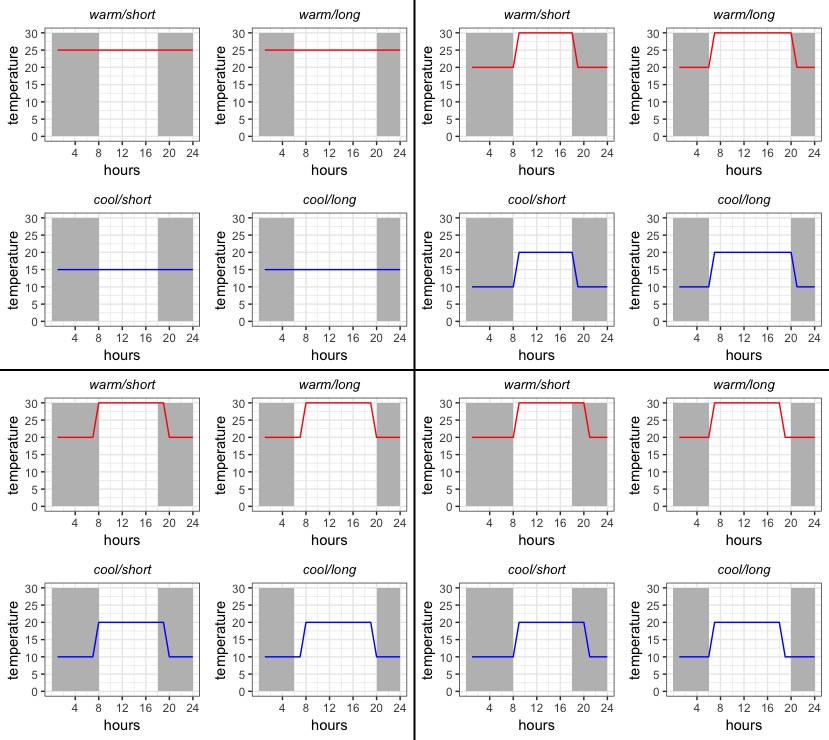
\includegraphics[width=\textwidth]{..//Plots/periodicity_figures/new_treats.jpeg}
    \caption{Experimental treatments}
    \label{fig:Figure 1}
\end{figure}

\begin{figure}[h!]
    \centering
 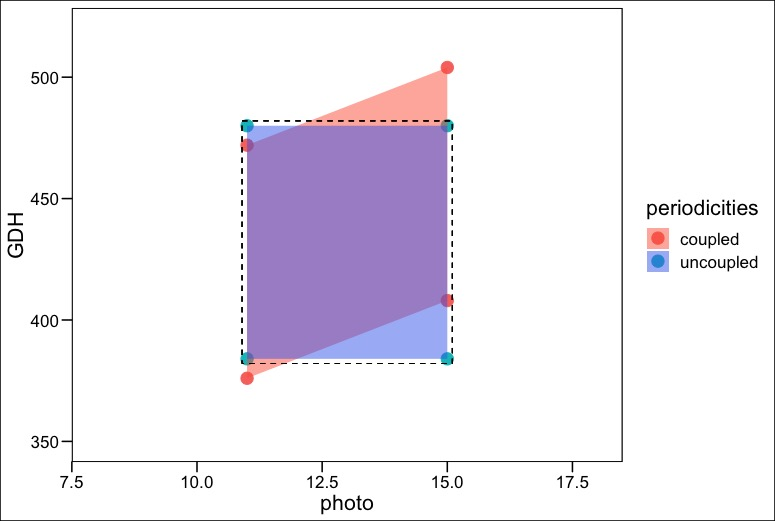
\includegraphics[width=\textwidth]{..//Plots/periodicity_figures/Uncoupled_coupled.jpeg}
    \caption{Experimental comparison all species}
    \label{fig:Figure 2}
\end{figure}

\begin{figure}[h!]
    \centering
 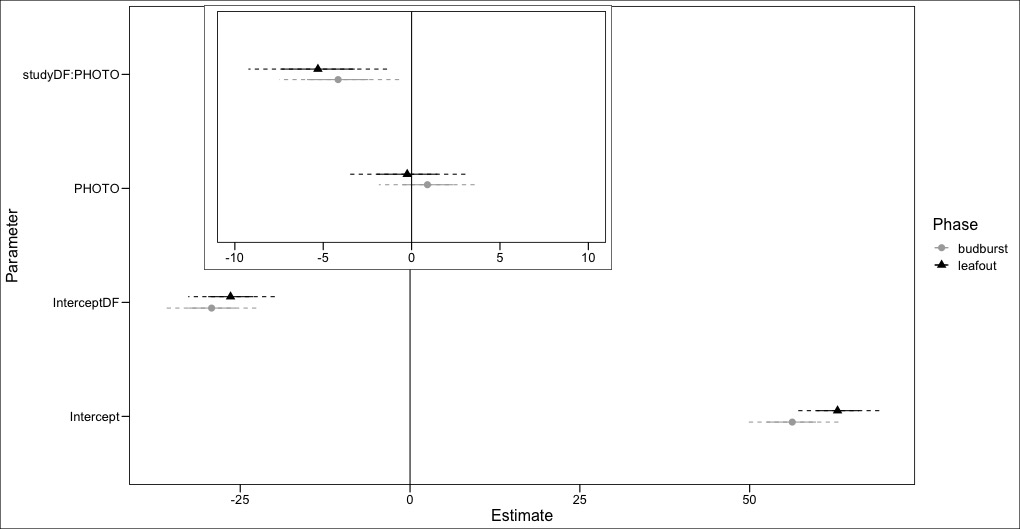
\includegraphics[width=\textwidth]{..//Plots/periodicity_figures/photothermo_allsps.jpeg}
    \caption{All species with partial pooling}
    \label{fig:Figure 3}
\end{figure}


\begin{figure}[h!]
    \centering
\begin{tabular}{|c|c|c|}
\hline
& predicted difference & observed difference (sd)\\
\hline
bud bust& 3.0 & -4.1575777(2.665567)\\
leaf out&3.0 & -5.3006250 (3.099359)\\
\hline
\end{tabular}
    \caption{Table}
    \label{fig:Figure 4}
\end{figure}

\end{document}



  % \begin{enumerate}
   %         \item Experiment testing interactions between photoperiod and forcing. 2 forcing treatment with different day and night values of 24/16, 20/12 \degree C, and 2 photoperiods of 11 and 15 day time hours. If we co-vary thermoperiod with photoperiod, rather than ending up with a 4-way factorial treatment design as intended, we sort of end up 4 separate treatments. Below based on 5 \degree C as threshold.
    %        \item Long/warm ends up with (24*15+16*9) 385 growing degree hours/ day
     %       \item Short/warm ends up with (19*11+11*13) 352 growing degree hours/ day
      %      \item Long/cool ends up with (15*15+7*9) 288 growing degree hours/day
       %     \item and Short cool ends up with (15*11+7*13) 256 growing degree hours/day.
        %    \item See? you can't tell the difference between the different photoperiod treatments vs. thermal sums.
         %   \item The alternative with be to vary thermperiod on its own independent cycle, eg. 12 hours of each day and night temperature. Then treatments at the same forcing level would have the same daily heat sum regardless of photoperiod.
    %    \end{enumerate}
    
    
